
\section{Cosmological distances} \label{sec:cosmological_distances}

Observables such as the redshift or distances are used in order to constrain the matter contents of the Universe as well as its expansion history and 
cosmological parameters. There are multiple ways one can define a distance in cosmology each relying on a different set of parameters. \\

\noindent \textbf{\underline{Physical distances}} \\

Under a FLRW metric, we can define the physical distance as the distance separating the observer and an event happening at $\chi$:
\begin{equation}
    d_p(\chi) = a_0 S_k(\chi)
\end{equation}
with $a_0$ being the scale factor at $t_0$. It is more practical to express $\chi$ as a function of the redshift since it is not a direct observable. If we consider a photon 
emitted at a time $t_e$ from the source object present at $\chi$ and recieved by the observer at $t_0$ then we get:
\begin{equation}
    \chi = c \int_{t_e}^{t_0} \frac{dt}{a(t)}
\end{equation}
By performing the following two variable changes:
\begin{equation}
    H = \frac{\dot{a}}{a} = \frac{1}{a} \frac{da}{dt} \Longleftrightarrow dt = \frac{da}{aH}
\end{equation}
\begin{equation}
    1+z = \frac{a_0}{a} \Longleftrightarrow dz = -\frac{a_0}{a^2}da
\end{equation}

We get:
\begin{equation}
    \chi = \frac{c}{a_0} \int_{0}^{z} \frac{dz'}{H(z')}
\end{equation}
Which gives us the following equation for the physical distance:
\begin{equation}
    \boxed{d_p(z) = a_0 S_k\left(\frac{c}{a_0} \int_{0}^{z} \frac{dz'}{H(z')}\right)}
\end{equation}
In a flat Universe, this expression is reduced to:
\begin{equation}
    d_p(z) = c \int_{0}^{z} \frac{dz'}{H(z')}
\end{equation}

In practice, this distance isn't directly measurable as it requires to measure the values $H$ at every redshift along the line of sight. However, other observable distances exist 
to which we can relate to the physical distance.\\

\noindent \textbf{\underline{Angular distances}} \\

We can firstly define the distance of an object based on its apparent size $D$ and angle $\Delta \theta$. We call this the angular distance and is defined as:
\begin{equation}
    \boxed{d_A = \frac{D}{\delta \theta} = a(t)S_k(\chi) = \frac{1}{1+z} a_0 S_k\left(\frac{c}{a_0} \int_{0}^{z} \frac{dz'}{H(z')}\right)}
\end{equation}
Therefore knowing the redshift, its apparent angle and size of an object gives us access to its distance.\\

\noindent \textbf{\underline{Luminosity distances}} \\

We can also determine the distance of an object by linking its intrinsic luminosity to its emitted flux at the surface. This defined as the luminosity distance $d_L$ and is given by:
\begin{equation}
    f = \frac{L}{4\pi d_L^2}
    \label{eqn:flux_dl}
\end{equation}
where $f$ is the surface flux and $L$ is the object's luminosity.\\

We need to account for the fact that the photons emitted are scattered on the surface $S$ of the object $S=4\pi a_0^2 S_k^2(\chi)$ as well as the fact that its energy ($\frac{hc}{\lambda}$) is 
is reduced by $1+z$ due to the cosmic expansion. The photons emitted during a duration of $\Delta t$ will be recieved during a diluted duration $\Delta t (1+z)$. This 
means that the observed luminosity will differ from the emitted luminosity giving us:
\begin{equation}
    L' = \frac{L}{(1+z)^2}
\end{equation}
where $L'$ is the luminosity seen by the observer. By definition, the surface flux is seen at an observer frame meaning:
\begin{equation}
    f=\frac{L'}{S} = \frac{L}{(1+z)^2 4\pi a_0^2 S_k^2(\chi) }
\end{equation}
We can then identify a formula for the luminosity distance that is redshift dependent:
\begin{equation}
    \boxed{d_L(z) = (1+z)a_0 S_k\left(\frac{c}{a_0} \int_{0}^{z} \frac{dz'}{H(z')}\right)}
    \label{eqn:distance_luminosity}
\end{equation}
We can see from the previous equations that:
\begin{equation}
    d_L(z) = d_A(z)(1+z)^2 = d_p(z)(1+z)
\end{equation}

At low redshift all three distance expression become equivalent and we can approximate it to:
\begin{equation}
    d_L(z) \approx \frac{cz}{H_0} \Leftrightarrow cz = v = H_0 d_L
\end{equation}
where we can see that we recover the Hubble law.\\


\begin{figure}[ht]
    \centering
    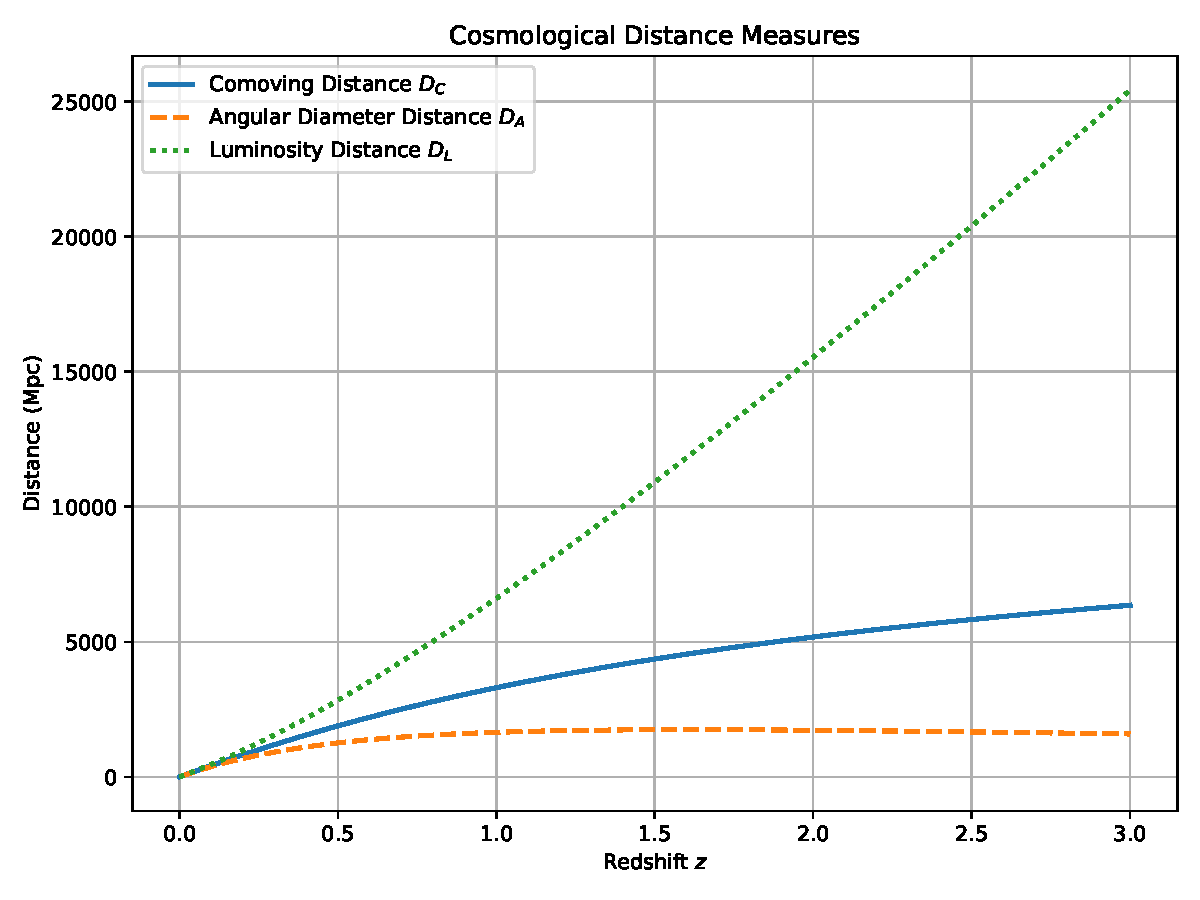
\includegraphics[width=1.0\textwidth]{MainLayout/Introduction_chapter/figures/distances.pdf}
    \caption{Different distances in cosmology plotted as a function of redshift for a flat $\Lambda$CDM with $H_0 = 70 \text{km.s}^{-1} \text{Mpc}^{-1}$ and $\Omega_m=0.3$.}
    \label{fig:hubble_riess}
\end{figure}

\section{Cosmological Observables}

In this section we will be briefly presenting some of the main observables that cosmologists are concerned with. \\

\subsection{The Cosmic Microwave Background}

During the radiation dominated era, the Universe was hot and dense, filled with a plasma of baryons and free electrons. Atoms could not form at that time because 
photons were energetic enough to ionise any neutral hydrogen immediately upon formation. As a result, baryonic matter remained tightly coupled to photons through 
Thomson scattering off free electrons. As the Universe expanded and cooled, photons eventually became insufficiently energetic to ionise hydrogen, allowing neutral atoms 
to form for the first time. This epoch is referred to as \textbf{recombination} and is associated with the decoupling of baryons and photons. The mean free path of 
photons then exceeded the Hubble radius, allowing them to travel freely across space without scattering. Today, these photons have been redshifted drastically due to the 
expansion of the Universe and are observed as a background of microwave radiation. We refer to this relic radiation as the Cosmic Microwave Background (CMB), and it 
constitutes our primary observational window onto the primordial Universe. The CMB was first discovered by Arno Penzias and Robert Wilson accidentally while calibrating 
an antenna for telecommunications and astronomy (\cite{Penzias_1965_a, Penzias_1965_b}). \\

The CMB has a nearly perfect blackbody spectrum with a mean temperature of $T_{CMB} = 2.7255 \pm 0.0006$ K (\cite{Fixsen_2009}) and temperature 
anisotropies at the level of $\Delta T / T \sim 10^{-5}$. The two-point correlation function of these anisotropies, equivalently described by the angular 
power spectrum $C_\ell$, encodes the imprint of primordial density perturbations consistent with a Gaussian random field (\cite{Planck_2018}), which later evolved 
into the large-scale structures we observe today. Secondary anisotropies, arising from effects such as gravitational lensing by galaxy clusters and inverse Compton 
scattering of CMB photons off hot intracluster gas (the Sunyaev-Zel'dovich effect), provide additional information on the late-time Universe. The polarisation of the 
CMB, decomposed into curl-free E-modes and divergence-free B-modes, further constrains inflationary models and provides a potential window onto primordial gravitational waves (\cite{Kamionkowski_1997}). \\

Through the detailed structure of the acoustic peaks in $C_\ell$, CMB observations allow precise constraints on multiple cosmological parameters, including $\Omega_m$, 
$\Omega_b$, $H_0$, $n_s$, and $A_s$ (\cite{Planck_2018_params}).\\

\begin{figure}[ht]
    \centering
    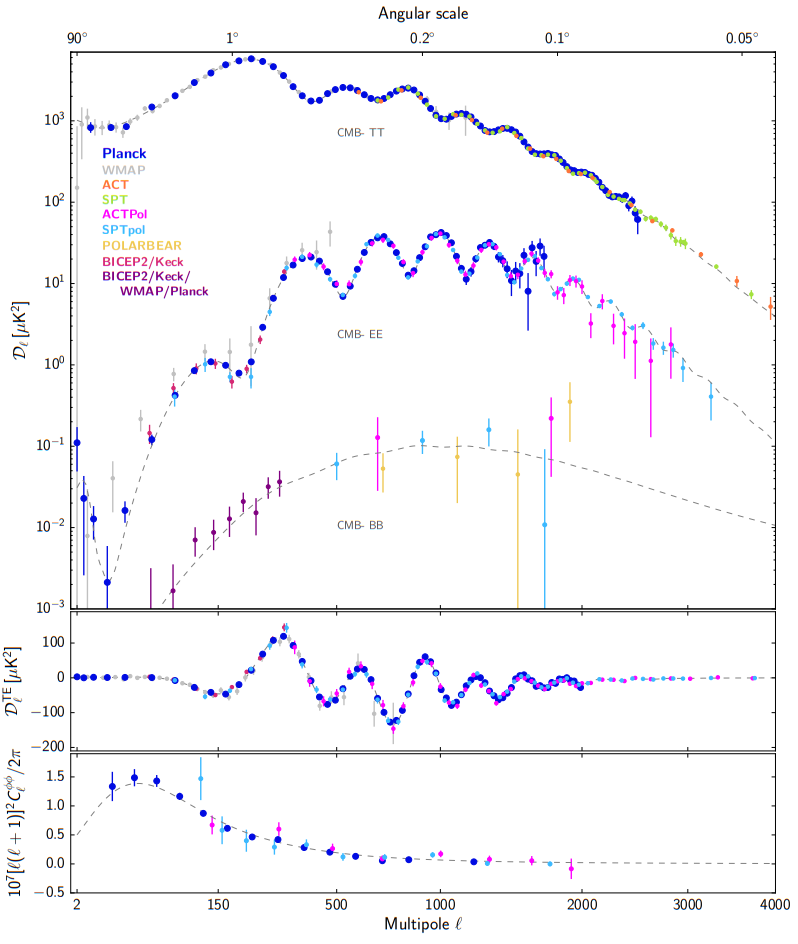
\includegraphics[width=0.7\textwidth]{MainLayout/Introduction_chapter/figures/angular_pk_cmb_.png}
    \caption{Compilation of CMB angular power spectrum measurements from \cite{Planck18_overview}.
    The upper panel shows the power spectra of the temperature and $E$-mode and $B$-mode polarization signals, the next panel the
    cross-correlation spectrum between $T$ and $E$, while the lower panel shows the lensing deflection power spectrum}
    \label{fig:pk_planck_angular}
\end{figure}

\subsection{Galaxy Surveys}

Galaxy surveys map the three-dimensional distribution of galaxies across large volumes of the Universe. Galaxies are biased tracers of the underlying matter 
distribution, and their spatial statistics allow us to infer a vast amount of information about the structure, dynamics, and history of the Universe. Surveys 
such as SDSS (\cite{York_2000}) and DESI (\cite{DESI_2016}) measure tens of millions of galaxies across a wide redshift range, from which significant cosmological 
constraints have been extracted. \\

\subsubsection{The Matter Power Spectrum}

A key statistical tool for analysing galaxy surveys is the matter power spectrum $P(k)$, defined as the variance of density fluctuations as a function of scale $k$:

\begin{equation}
    \langle \delta(\mathbf{k})\delta^*(\mathbf{k}') \rangle = 
    (2\pi)^3 \mathcal{P}(k)\,\delta^{(3)}_D(\mathbf{k} - \mathbf{k}')
\end{equation}

The shape and amplitude of $\mathcal{P}(k)$ depend directly on cosmological parameters. The primordial power spectrum can be related to late-time observations through the 
transfer function (\cite{Eisenstein_Hu_1998}):

\begin{equation}
    \mathcal{P}(k) = A_s \left(\frac{k}{k_*}\right)^{n_s - 1} T^2(k)\,D_1^2(z)
\end{equation}

where $k_* = 0.05\,\mathrm{Mpc}^{-1}$ is the pivot scale at which the primordial amplitude $A_s$ is defined (\cite{Planck_2018_inflation}), $T(k)$ is the transfer 
function encoding the scale-dependent evolution of perturbations through radiation domination, and $D_1(z)$ is the linear growth factor describing the 
growth of structure during matter domination. \\

\begin{figure}[ht]
    \centering
    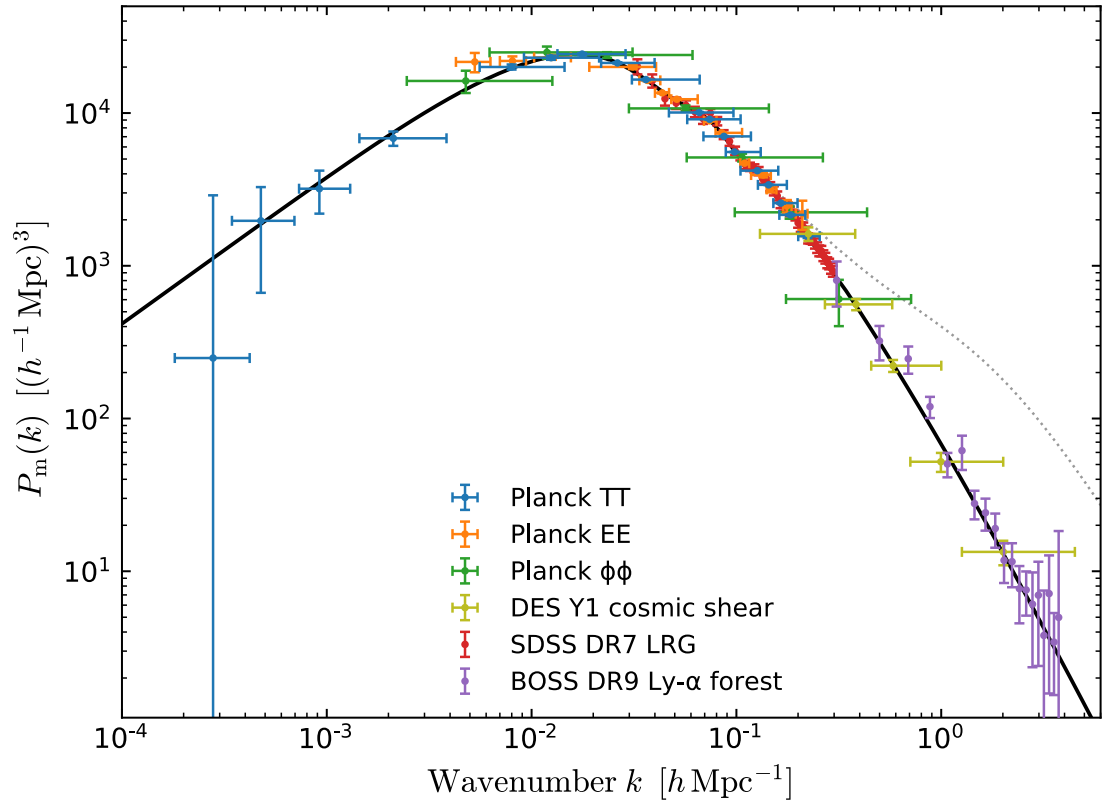
\includegraphics[width=1.0\textwidth]{MainLayout/Introduction_chapter/figures/matter_pk_planck.png}
    \caption{Linear-theory matter power spectrum (at $z=0$) inferred from different cosmological probes taken from \cite{Planck18_overview}.}
    \label{fig:pkm_planck}
\end{figure}

\subsubsection{Baryon Acoustic Oscillations}

Baryon Acoustic Oscillations (BAO) are a feature in the matter clustering that corresponds to the imprint of sound waves propagating through the baryon-photon 
plasma in the early Universe. The radiation pressure of the hot plasma drove acoustic oscillations at a sound speed of $c_s \simeq c/\sqrt{3}$. These 
oscillations were frozen in at the \textbf{drag epoch} $z_d \approx 1060$, shortly after photon decoupling at $z_* \approx 1100$, when baryons decoupled from the 
photon fluid and the sound waves could no longer propagate. The comoving distance these sound waves had travelled by that time defines the \textbf{sound horizon}:

\begin{equation}
    r_s(z_d) = \int_{z_d}^{\infty} \frac{c_s(z)}{H(z)}\,dz \approx 147\,\mathrm{Mpc}
\end{equation}

This characteristic scale is imprinted in the distribution of matter as a preferred separation between galaxies, appearing as a distinct peak in the two-point 
correlation function $\xi(r)$ at $r \approx 147$ Mpc, or equivalently as oscillations in $P(k)$. The BAO scale thus defines a \textbf{standard ruler} that 
can be measured at different redshifts to constrain the expansion history of the Universe through $H(z)$ and the angular diameter distance $D_A(z)$ 
(\cite{Eisenstein_2005}, \cite{Blake_2003}). \\

\begin{figure}
    \begin{subfigure}{.5\textwidth}
      \centering
      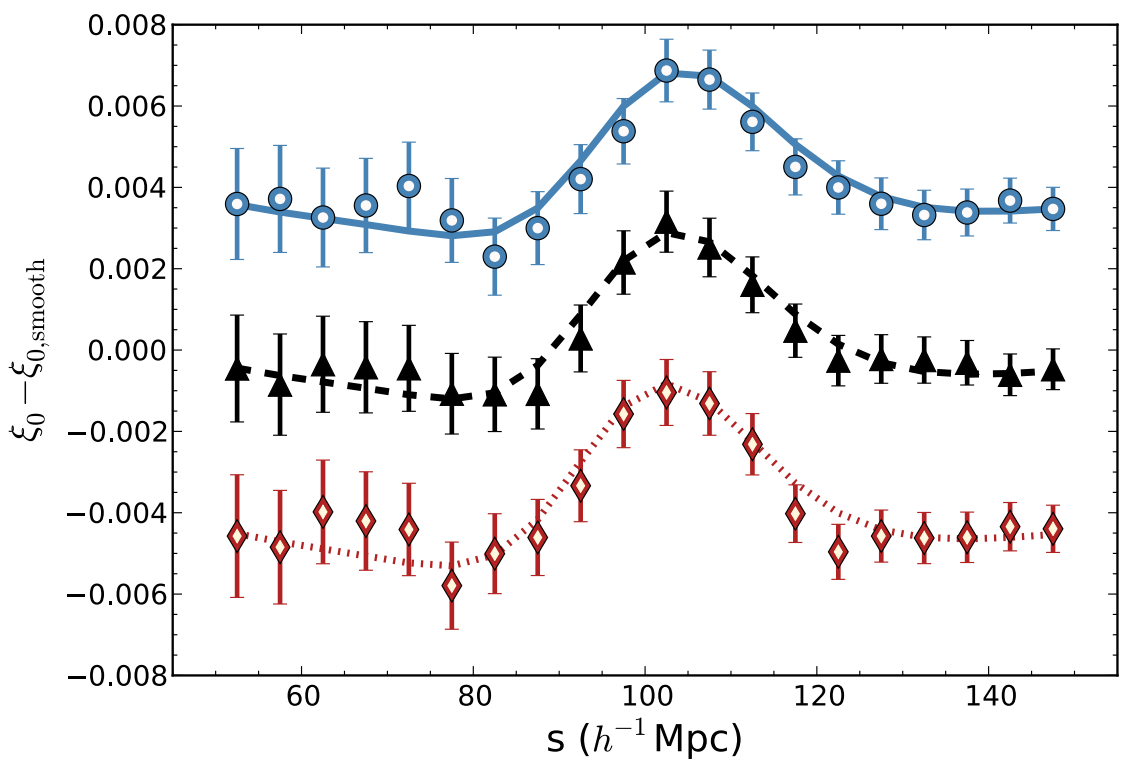
\includegraphics[width=1.\linewidth]{MainLayout/Introduction_chapter/figures/bao_corr_sdss.png}
      \caption{}
      \label{fig:bao_a}
    \end{subfigure}%
    \begin{subfigure}{.5\textwidth}
      \centering
      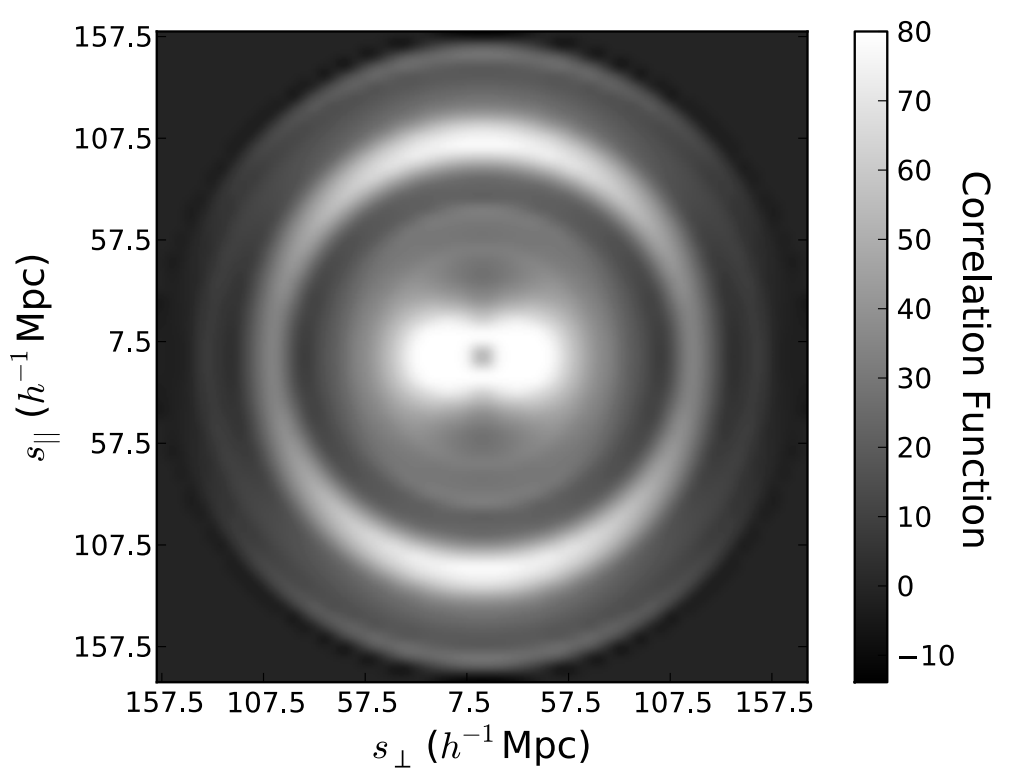
\includegraphics[width=1.\linewidth]{MainLayout/Introduction_chapter/figures/bao_corr_3d_sdss.png}
      \caption{}
      \label{fig:bao_b}
    \end{subfigure}
    \caption{BAO signals in the measured correlation functions from SDD (\cite{Alam_2017}). On the left is the smoothed prediction of the best-fitted model. On the right 
    the redshift bins are decomposed into the component of the separations transverse to and along the line of sight at $0.4<z<0.6$.}
    \label{fig:bao}
\end{figure}

\subsubsection{Redshift Space Distortions}

Galaxies are observed in redshift space rather than real space. Their peculiar velocities along the line of sight distort their apparent positions, producing 
anisotropies in the observed galaxy clustering. On large scales, coherent infall of galaxies into overdensities causes an apparent compression of structures along 
the line of sight, known as the \textbf{Kaiser effect} (\cite{Kaiser_1987}). On small scales, the virial motions of galaxies within collapsed structures produce 
an elongation of structures along the line of sight, known as the \textbf{Fingers of God} effect (\cite{Jackson_1972}). \\

The amplitude of these distortions depends on the rate of structure growth, encapsulated in the parameter $f\sigma_8$, where $f = d\ln D_1/d\ln a \approx 
\Omega_m(z)^{0.55}$ is the growth rate predicted by General Relativity and $\sigma_8$ is the amplitude of matter fluctuations on scales of $8\,h^{-1}$ Mpc. 
Modified gravity theories predict different values of $f$, making measurements of $f\sigma_8$ a direct test of GR on cosmological scales (\cite{Guzzo_2008}, 
\cite{Planck_2018_params}). \\

\subsection{Type Ia Supernovae}

As discussed in Section \ref{sec:cosmological_distances}, it is possible to obtain the distance of an object through its luminosity. However, measuring the intrinsic luminosity 
of celestial objects is a difficult task in itself. Type Ia Supernovae are thermonuclear explosions involving white dwarf stars that 
are \textbf{standardizable candles}, meaning they're characterized by a reproducible intrinsic luminosity. By measuring their apparent brightness as a function of redshift, 
one can reconstruct the luminosity distance-redshift relation $d_L(z)$ and constrain the expansion history of the Universe. 
This led to the discovery of the accelerated expansion of the Universe (\cite{Riess_1998}, \cite{Perlmutter_1999}). A detailed discussion of Type Ia 
Supernovae and their use as cosmological probes is presented in Chapter 2. \\

\subsection{Gravitational Lensing}

According to general relativity, mass curves spacetime and light follows the geodesics of that curved geometry. As a result, the path of photons is deflected 
when passing near massive objects, a phenomenon known as gravitational lensing. In a cosmological context, this deflection can be derived from the geodesic equation 
applied to the perturbed FLRW metric, and it provides a direct probe of the total matter distribution,both baryonic and dark, along the line of sight. \\

Two main regimes of gravitational lensing are relevant for cosmology. \textbf{Strong lensing} occurs in the vicinity of objects with deep gravitational potentials, such 
as massive galaxy clusters, producing dramatic and easily identifiable distortions such as multiple images, giant arcs, and Einstein rings. It provides precise 
measurements of the mass distribution of individual clusters. \textbf{Weak lensing} operates in the regime where the distortion of any individual background source is 
too small to be detected — the induced ellipticity is much smaller than the intrinsic ellipticity of a galaxy \cite{Bartelmann_2001}. However, the lensing signal can be recovered statistically 
by measuring the coherent distortion of the shapes of large samples of background galaxies, an effect known as \textbf{cosmic shear} $\gamma$. \\

Since lensing responds to all matter along the line of sight, cosmic shear surveys provide a direct measurement of the projected matter distribution. 
The amplitude of the cosmic shear signal is sensitive to both the amplitude of matter fluctuations $\sigma_8$ and the matter density $\Omega_m$, but these two parameters are largely degenerate in lensing observations. This degeneracy is 
characterised by the parameter $S_8 = \sigma_8(\Omega_m / 0.3)^{0.5}$,  which current surveys constrain to percent-level precision (\cite{KiDS_2021} \cite{DES_Y3_2022}).\\

\begin{figure}[ht]
    \centering
    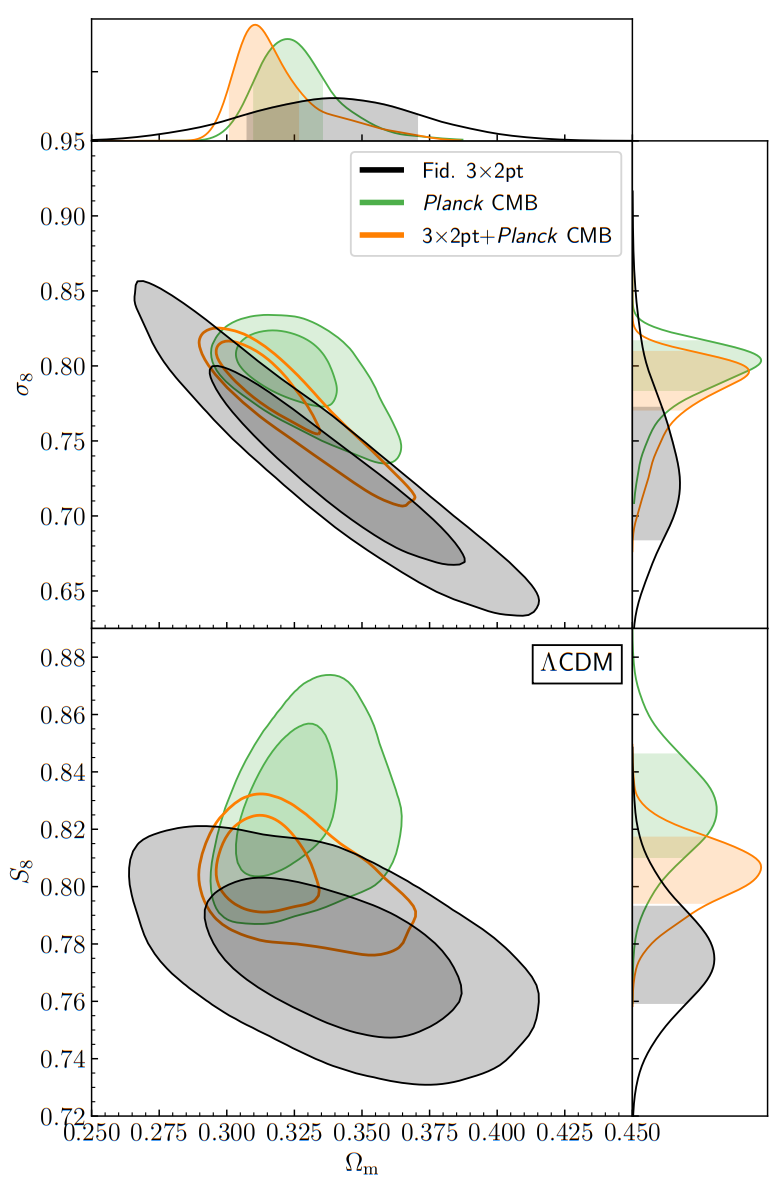
\includegraphics[width=0.6\textwidth]{MainLayout/Introduction_chapter/figures/lensing_constraints_.png}
    \caption{A comparison of the marginalized parameter constraints in the $\Lambda$CDM model from the Dark Energy Survey (\cite{DES_Y3_2022}) with predictions from Planck CMB data (no lensing; green). There is also the fiducial cosmology 3x2pt (black) and the combined Y3 3x2pt and Planck (orange) results.}
    \label{fig:lensing}
\end{figure}


\subsection{The Lyman-$\alpha$ Forest}

When observing the spectra of distant quasars, a dense series of absorption lines is observed, a feature known 
as the \textbf{Lyman-$\alpha$ forest}. These absorption lines are produced by neutral hydrogen clouds in the intergalactic medium (IGM) through which the quasar 
photons pass on their way to the observer, typically at redshifts $2 \lesssim z \lesssim 5$. Each absorbing cloud at redshift $z$ produces an absorption line at 
an observed wavelength:
\begin{equation}
    \lambda_{obs} = 1216\,(1+z)\;\text{\AA}
\end{equation}
where $1216\,\text{\AA}$ is the restframe Lyman-$\alpha$ wavelength. It's possible to show that the neutral hydrogen fraction in the IGM traces the 
underlying total matter density field, making the Lyman-$\alpha$ forest an effective map of the matter distribution along the line of sight 
(\cite{Gunn_1965}). \\

The cosmological information in the Lyman-$\alpha$ forest is extracted through the power spectrum of the transmitted flux fluctuations, which can be directly related 
to the three-dimensional matter power spectrum (\cite{Croft_1998}). A particularly powerful feature of this probe is that it is sensitive to scales 
$k \sim 0.1$--$10\,h\,\mathrm{Mpc}^{-1}$ at high redshift, well beyond the reach of galaxy surveys, making it highly complementary to both CMB and galaxy clustering 
measurements. This sensitivity to small scales and high redshifts allows the Lyman-$\alpha$ forest to constrain the sum of neutrino masses $\sum m_\nu$ through 
the small-scale suppression of the power spectrum (\cite{Palanque_2015}), the spectral index $n_s$ and the BAO standard ruler at $z \sim 2.3$ 
(\cite{Delubac_2015}).\\

\begin{figure}[ht]
    \centering
    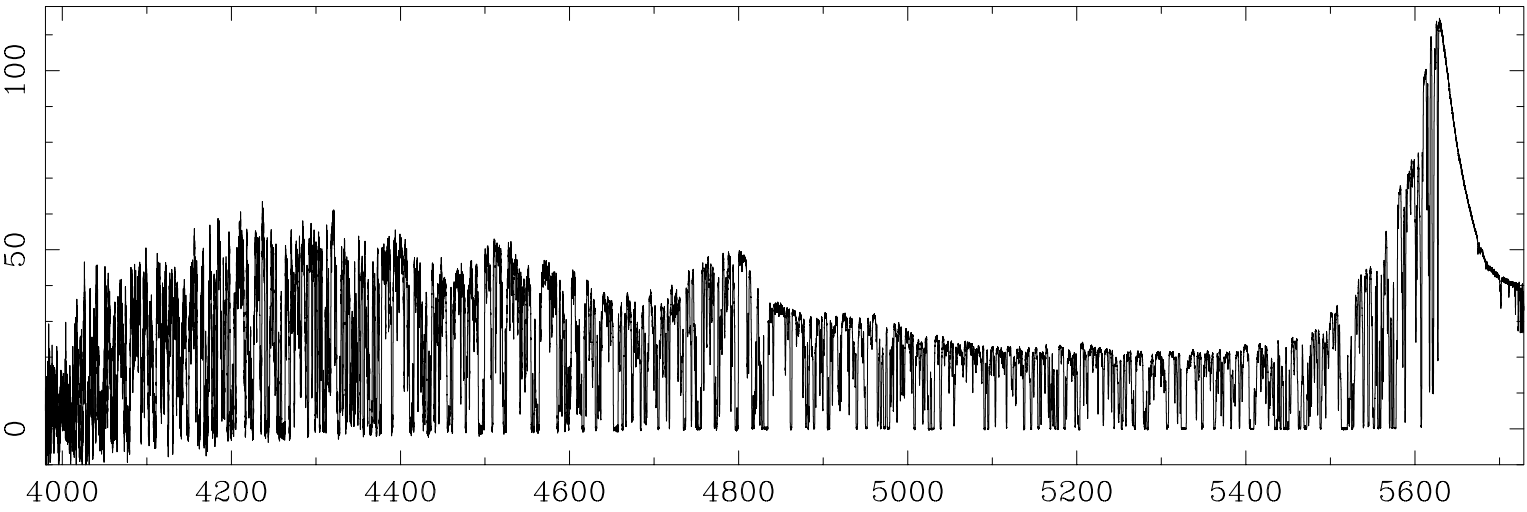
\includegraphics[width=1.0\textwidth]{MainLayout/Introduction_chapter/figures/lya.png}
    \caption{High resolution spectrum of the Lyman-$\alpha$ forest part of a quasar measured at $z=3.63$ taken with the HIRES spectrograph on the 10 m Keck telescope in Hawaï.}
    \label{fig:lyman_alpha}
\end{figure}
